\documentclass[../../main.tex]{subfiles}

\begin{document}

\begin{longtable}{| p{.20\textwidth} | p{.80\textwidth} |} 
\hline
    Kratak opis &  Administrator u sistemu unosi izmene u informacijama o takmičenju. Ukoliko želi šalje i propratno obaveštenje prijavljenima, trenerima i/ili klijentima. Baza se ažurira.\\ 
\hline    
    Učesnici & Administrator - Želi da izmeni podatke o takmičenju. \\
\hline
   Preduslovi & \begin{enumerate}
       \item Sistem je u funkciji.
       \item Postoji zakazano takmičenje.
       \item Administrator ima pristup sistemu.
   \end{enumerate}\\
\hline  
    Postuslovi & Baza podataka je ažurirana.\\
\hline
    Osnovni tok & \begin{enumerate}
        \item Administrator u delu sistema za upravljanje takmičenjima pored željenog takmičenja bira dugme "Izmeni".
        \item Sistem prikazuje postojeće podatke i polja za unos izmene.
        \item Administrator unosi izmene i po završetku bira dugme "Sačuvaj izmene".
        \item Sistem proverava ispravnost unetih podataka. Sistem obaveštava administratora o ispravnosti podataka i nudi mu da pošalje obaveštenje o izmenama.
        \item Administrator bira grupe korisnika koje želi da obavesti i unosi tekst poruke. Bira dugme "Obavesti".
        \item Sistem šalje mejlove. 
        \item Sistem čuva izmene i obaveštava administratora da je izmena uneta.
    \end{enumerate}\\
\hline
    Alternativni tokovi & \begin{itemize}
        \item[A1] Pad sistema: Administrator resetuje sistem i ponovo se loguje. Slučaj se nastavlja na koraku 1.
        \item[A5] Podaci nisu validni: Sistem obaveštava administratora koji uneti podaci nisu validni. Slučaj se nastavlja na koraku 2.
        \item[A6] Administrator ne želi nikoga da obavesti: Administrator bira dugme "Prekoči obaveštenja". Slučaj se nastavlja na koraku 8.
    \end{itemize}\\
\hline
    Podtokovi & /\\
\hline
    Specijalni zahtevi & /\\
\hline
    Dodatne informacije & /\\
\hline
\caption{Izmena informacija o takmičenju} % needs to go inside longtable environment    
\end{longtable}

\begin{figure}[!ht]
\begin{center}
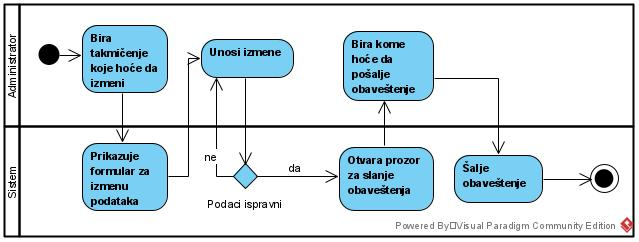
\includegraphics[scale=0.55]{sections/images/dijagram_aktivnosti_izmena_podataka_takmicenje.jpg}
\end{center}
\caption{Dijagram aktivnosti za izmenu informacija o takmičenju}
\label{fig:kontekst}
\end{figure}

\end{document}